\documentclass[a4paper, 8pt]{book}
\usepackage[margin=0.8cm, includefoot, includehead]{geometry}

\usepackage{url}
\usepackage{epsfig}
\usepackage{graphics}

\usepackage{fancyhdr}
\fancyhf{} % clear all header and footers
\renewcommand{\headrulewidth}{0pt} % remove the header rule
\fancyhead[R]
{
	\ifodd\value{page}
		\thepage
	\else
		\hfill
	\fi
}
\fancyfoot[R]
{
	\ifodd\value{page}
		\hfill
	\else
		\thepage
	\fi
}

\pagestyle{fancy}
\fancypagestyle{plain}{%
	\fancyhf{}%
	\renewcommand{\headrulewidth}{0pt}%
	\fancyhead[R]
	{
		\ifodd\value{page}
			\thepage
		\else
			\hfill
		\fi
	}
	\fancyfoot[R]
	{
		\ifodd\value{page}
			\hfill
		\else
			\thepage
		\fi
	}
}

\usepackage{graphicx}
\usepackage{parskip}
\usepackage[utf8]{inputenc}
\usepackage{float}
\usepackage{calc}
\usepackage{subcaption}
\usepackage[numbers]{natbib}
\usepackage{algorithm}
\usepackage[noend]{algpseudocode}
\usepackage{amsmath}
\usepackage[numbib,nottoc]{tocbibind}
\usepackage[table,xcdraw]{xcolor}
\usepackage{multirow}
\usepackage[brazil]{babel}
\usepackage[pages=some]{background}
\usepackage{afterpage}
\usepackage{color}
\usepackage{kantlipsum}
\usepackage[sfdefault,light]{roboto}  %% Option 'sfdefault' only if the base font of the document is to be sans serif
\usepackage[T1]{fontenc}
\usepackage{multicol}
\usepackage{ragged2e}
\usepackage{tabu}

\usepackage[toc]{multitoc}
\renewcommand*{\multicolumntoc}{2}
% \setlength{\columnseprule}{0.5pt}

\usepackage{titlesec}
\titlespacing*{\section}
{0cm}{0.1cm}{0cm}
\titlespacing*{\subsection}
{0cm}{0cm}{0cm}

\usepackage{hyperref}
\hypersetup{
    colorlinks,
    citecolor=black,
    filecolor=black,
    linkcolor=black,
    urlcolor=black
}

% 
\usepackage{environ}
\usepackage{pgfkeys}
\makeatletter
\newlength{\ae@width}
\newlength{\ae@hoffset}
\newlength{\ae@topsep}
\newlength{\ae@botsep}
\newlength{\ae@colheight}
\newlength{\ae@colsep}
\newlength{\ae@colrulewidth}
\pgfkeys{/ae/multi/columns/.cd,
  width/.code=\setlength\ae@width{#1},
  hoffset/.code=\setlength\ae@hoffset{#1},
  topsep/.code=\setlength\ae@topsep{#1},
  botsep/.code=\setlength\ae@botsep{#1},
  height/.code=\setlength\ae@colheight{#1},
  colsep/.code=\setlength\ae@colsep{#1},
  colrulewidth/.code=\setlength\ae@colrulewidth{#1},
}

\NewEnviron{aemulticol}[1][]
  {\pgfkeys{/ae/multi/columns/.cd,
    topsep=0cm,
    botsep=0ex,
    hoffset=0in,
    width=2in,
    height=0in,
    colsep=0.3cm,
    colrulewidth=0.4pt,
    #1}%%
   \vspace{\ae@topsep}\par
   \noindent
   \hspace*{\ae@hoffset}%%
   \makebox[0pt][l]{\ae@set@multi@cols}%%
   \vspace{\ae@botsep}\par
  }

\def\ae@set@multi@cols{%%
  \setbox0=\vbox{%%
    \hsize=\ae@width
    \BODY}%%
  \splittopskip=0pt
  \vbadness=10000\relax
  \ae@build@column
}

\def\ae@build@column{%%
  \setbox2=\vsplit0 to \ae@colheight 
  \vtop{%%
    \hrule height0pt 
    \unvbox2
  }%%
  \ifvoid0\relax\else
    \hspace{\dimexpr(\ae@colsep-\ae@colrulewidth)/2}%%
    % \vrule width \ae@colrulewidth
    \hspace{\dimexpr(\ae@colsep-\ae@colrulewidth)/2}%%
    \expandafter\ae@build@column
  \fi}  

\makeatother
% 

\usepackage{tikz}
\usetikzlibrary{calc}

\usepackage{tocloft}
\setlength{\cftbeforesecskip}{0.1cm}

\definecolor{section_color}{RGB}{227, 170, 84}
\definecolor{subsection_color}{RGB}{125, 87, 68}

\newcommand*{\sectioncolor}{section_color}
\newcommand*{\sectionformat}{\color{\sectioncolor}}

\newcommand*{\subsectioncolor}{subsection_color}
\newcommand*{\subsectionformat}{\color{\subsectioncolor}}

\graphicspath{{pictures/}}

\backgroundsetup
{
	scale = 1,
	color = black,
	opacity = 1.0,
	angle = 0,
	contents = 
	{
  		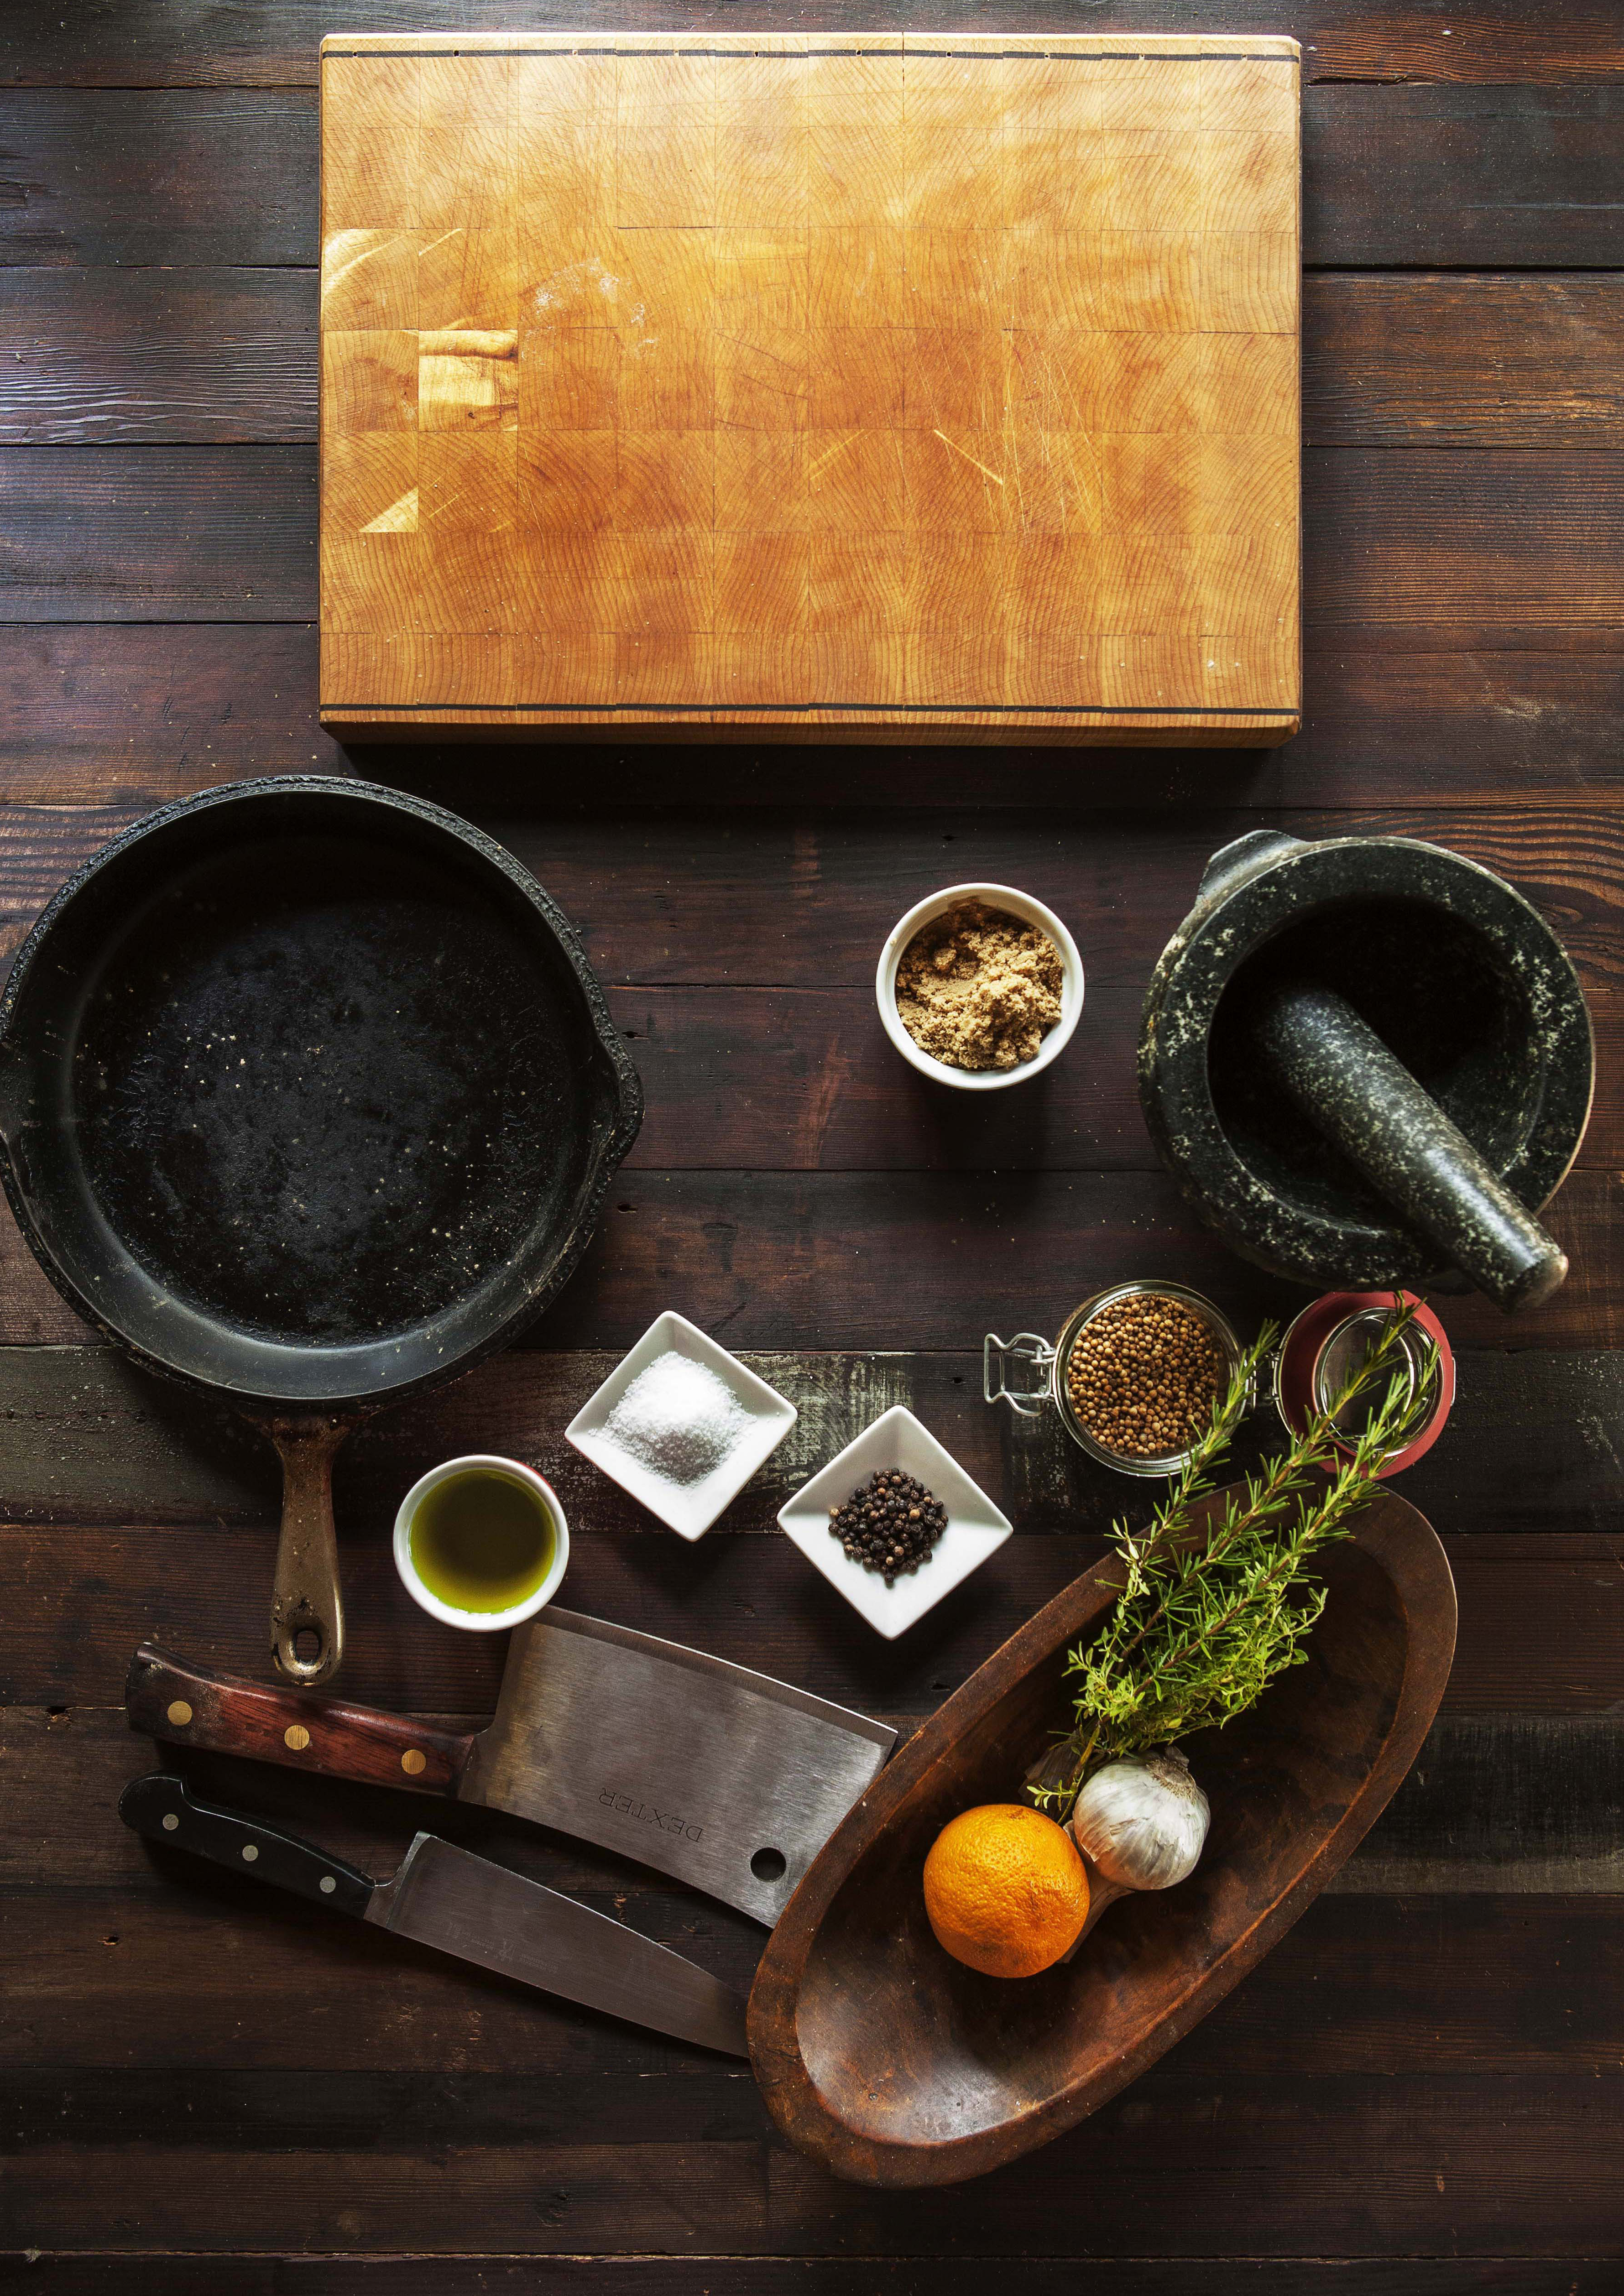
\includegraphics[width=\paperwidth,height=\paperheight]{cover.jpg}
  	}
}

\title
{
	\vspace*{-12.8cm}
	\scalebox{1.2}
	{
		\textbf{E aí, como estamos de macarrão?}
	}
	\scalebox{0.84}
	{
		Um guia de receitas que deram certo
	}
}
\author
{
	\\[3.0cm]
	\centering
	\scalebox{1.2}
	{
	    \begin{tabular}{cc}
			\multicolumn{2}{c}{
				Cobaias
			}
			\\[0.15cm]
			\multicolumn{2}{c}{
				Leila Barreto \& Thiago Lobo
			}
		\end{tabular}
	}
}
\date{}

\begin{document}
	\BgThispage
	\maketitle
		
	\newpage
	\vspace*{-3cm}
	\tableofcontents
	
	\newpage
\noindent
\vspace*{-2.0cm}
\section*{\sectionformat Nome da Receita}
\addcontentsline{toc}{section}{Nome da Receita}
\vspace*{-0.1cm}
\begin{aemulticol}[width=0.495\textwidth,height=0.545\textheight]
	\begin{tabu} to 0.5\linewidth {X[l]X[r]}
	   \textit{Serve $3$ pessoas} & \textit{$430$ kcal}
	\end{tabu}\\
	\rule[0.5ex]{0.5\linewidth}{1pt}
	
	\vspace*{-0.3cm}
	\subsection*{\subsectionformat Ingredientes}
	\vspace*{-0.15cm}
	\begin{tabu} to 0.5\linewidth {X[l]X[l]}
	   $\bullet$ ingrediente com nome muito grande grande demais mesmo que cai pra outra linha & $\bullet$ ingrediente\\
	   $\bullet$ ingrediente & $\bullet$ ingrediente\\
	   $\bullet$ ingrediente & $\bullet$ ingrediente\\
	   $\bullet$ ingrediente & $\bullet$ ingrediente\\
	   $\bullet$ ingrediente & $\bullet$ ingrediente
	\end{tabu}

	\vspace*{-0.15cm}
	\subsection*{\subsectionformat Modo de Preparo}
	\vspace*{-0.15cm}
	$1.$  Passo 1\\
	$2.$  Passo 2\\
	$3.$  Passo 3\\
	$4.$  Passo 4\\
	$5.$  Passo 5\\
	$6.$  Passo 6\\
	$7.$  Passo 7\\
	$8.$  Passo 8\\
	$9.$  Passo 9\\
	$10.$ Passo 10\\
	$11.$ Passo 11\\
	$12.$ Passo 12\\
	$13.$ Passo 13\\
	$14.$ Passo 14\\
	$15.$ Passo 15\\
	$16.$ Passo 16\\
	$17.$ Passo 17\\
	$18.$ Passo 18\\
	$13.$ Passo 13\\
	$14.$ Passo 14\\
	$16.$ Passo 16\\
	$17.$ Passo 17\\
	$18.$ Passo 18\\
	$13.$ Passo 13\\
	$14.$ Passo 14\\
	$16.$ Passo 16\\
	$17.$ Passo 17\\
	$18.$ Passo 18\\
	$13.$ Passo 13\\
	$14.$ Passo 14\\
	$15.$ Passo 15\\
	$16.$ Passo 16\\
	$17.$ Passo 17\\
	$18.$ Passo 18\\
	$19.$ Passo 19	

	\vspace*{-0.15cm}
	\subsection*{\subsectionformat Dicas}
	\vspace*{-0.15cm}
	
	$\bullet$ Dica 1\\
	$\bullet$ Dica 2\\
	$\bullet$ Dica 3
	
	\vspace*{-0.15cm}
	\subsection*{\subsectionformat História}
	\vspace*{-0.15cm}
	\textit{Essa receita foi criada para testar o layout do livro e infelizmente, provavelmente nunca será feita. Coitada da receita.}
\end{aemulticol}
\begin{tikzpicture}[remember picture, overlay]
\node[anchor = south, inner sep = 0pt, outer sep = 0pt] at (current page.south) 
{
	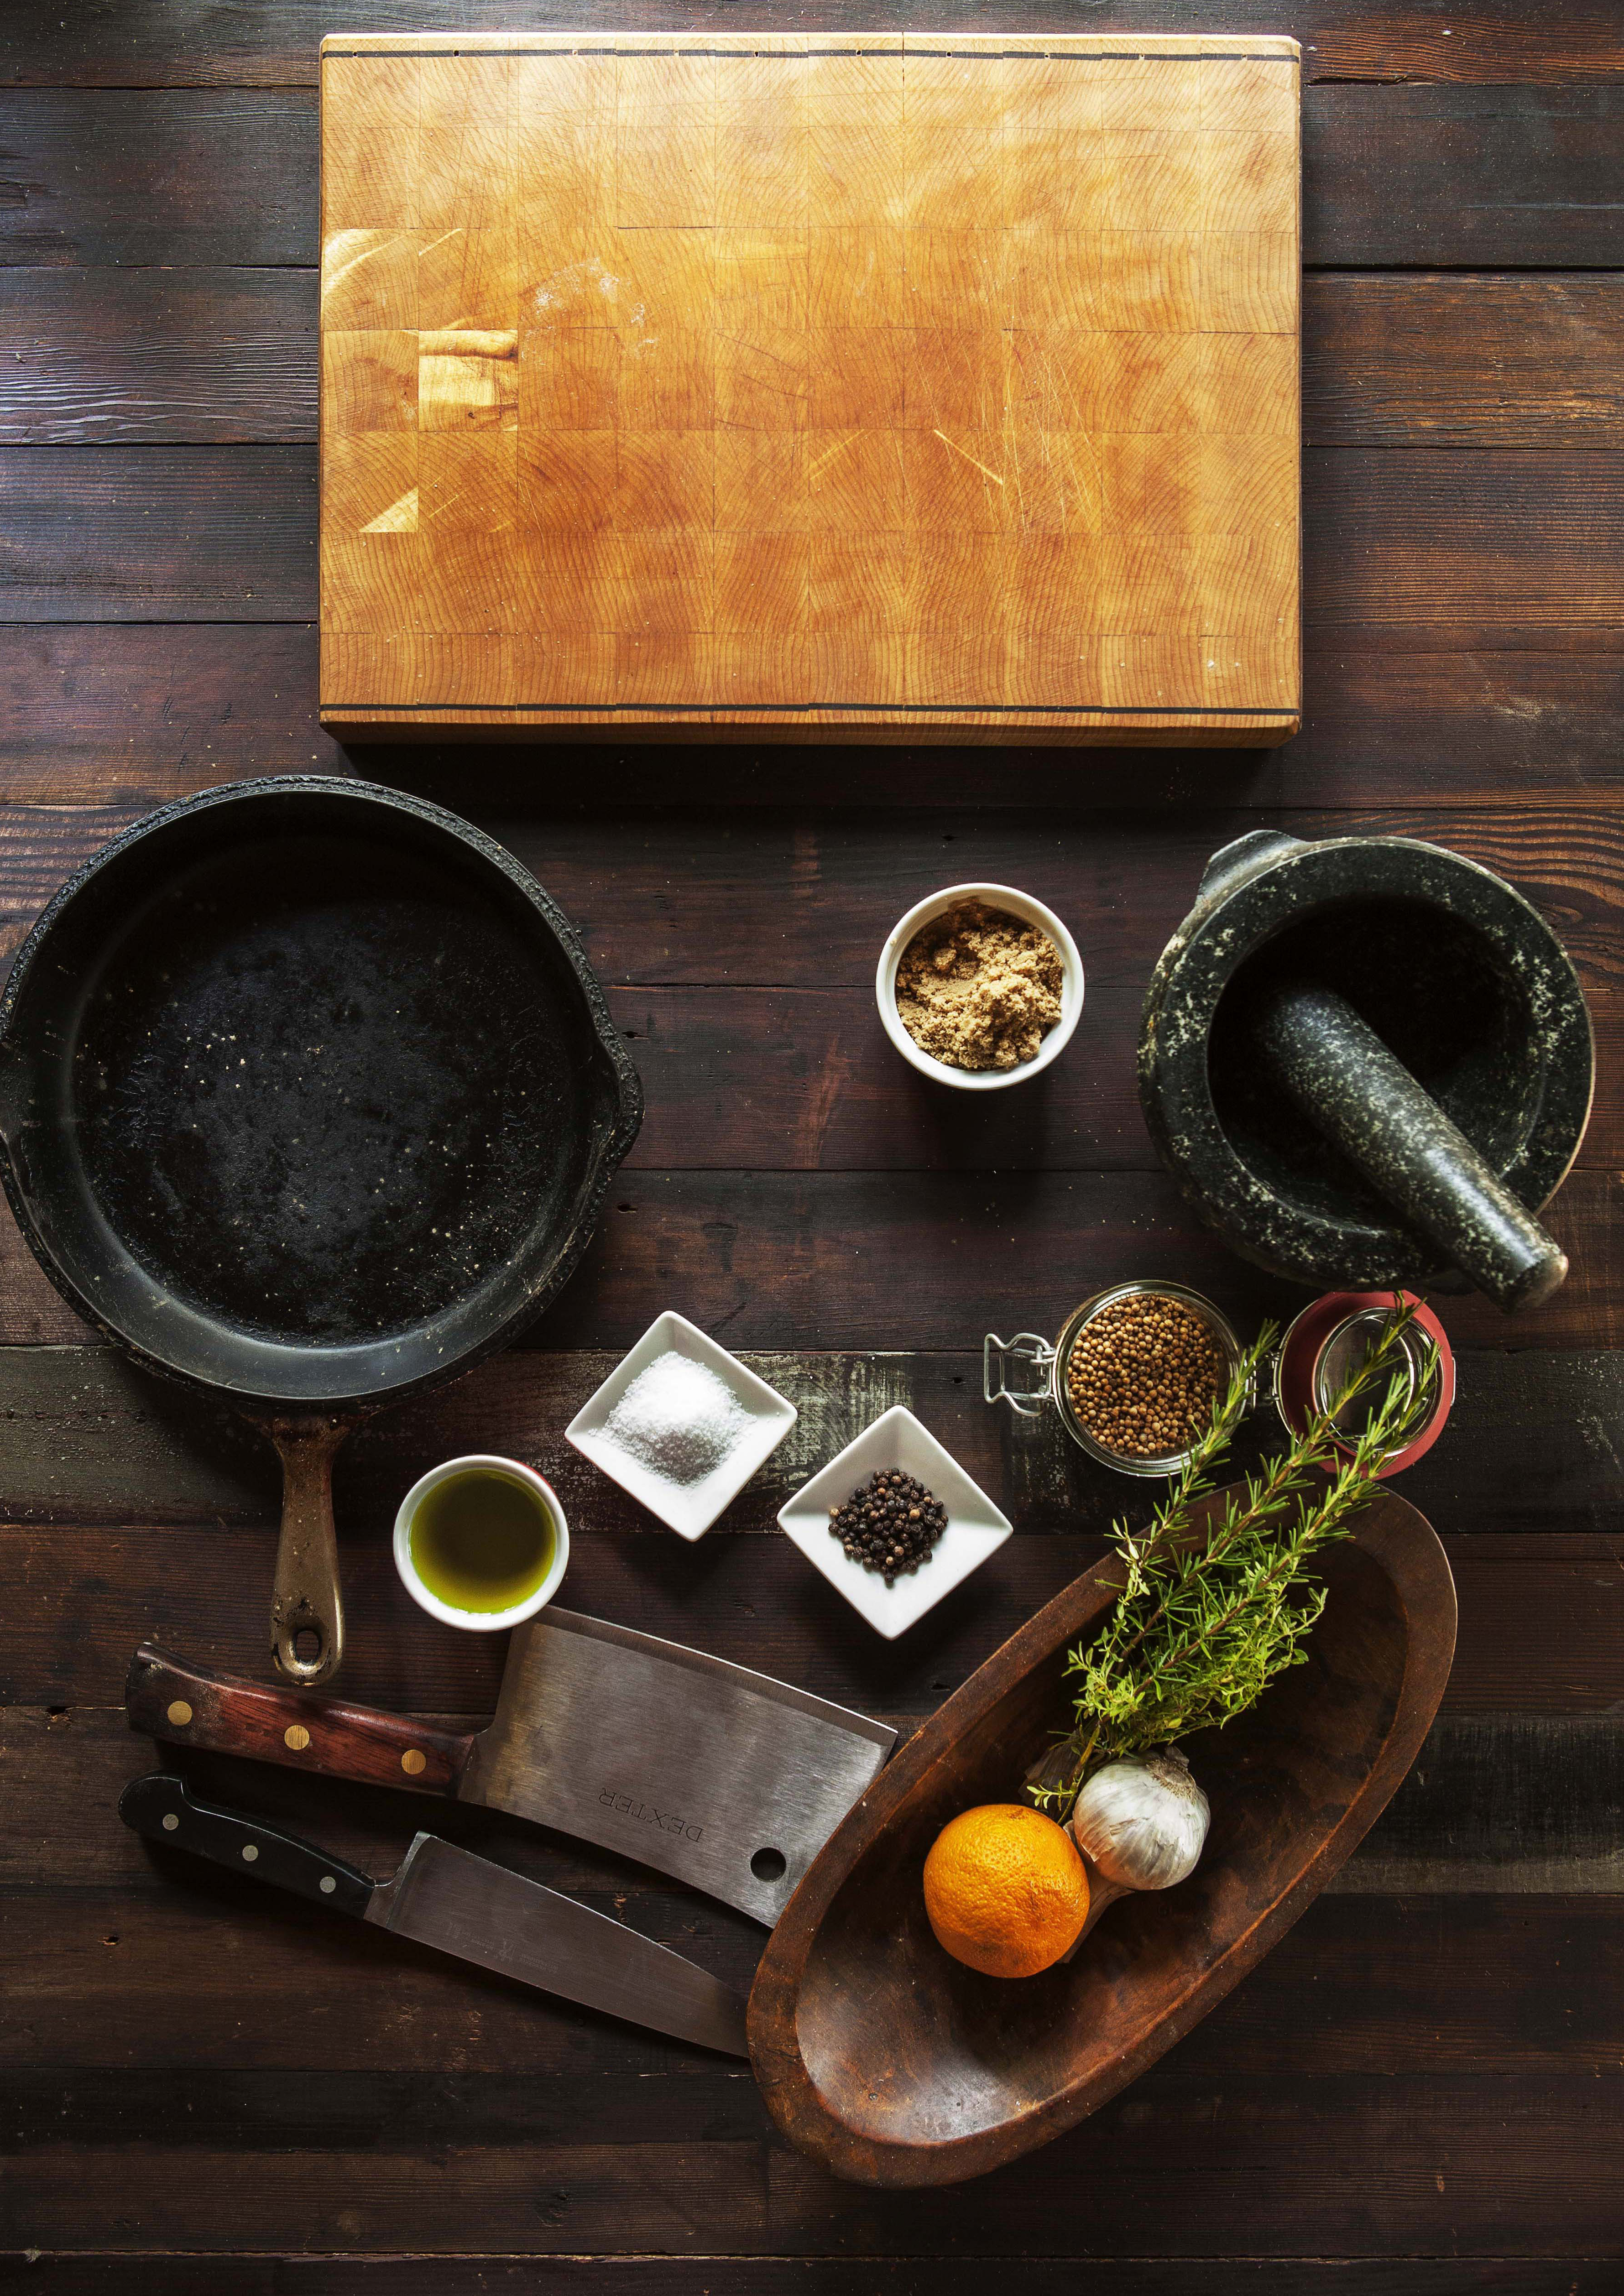
\includegraphics[width=\paperwidth, height=0.45\paperheight]{cover.jpg}
};
\end{tikzpicture}
	\newpage
\noindent
\begin{tikzpicture}[remember picture, overlay]
\node[anchor = north, inner sep = 0pt, outer sep = 0pt] at (current page.north) 
{
	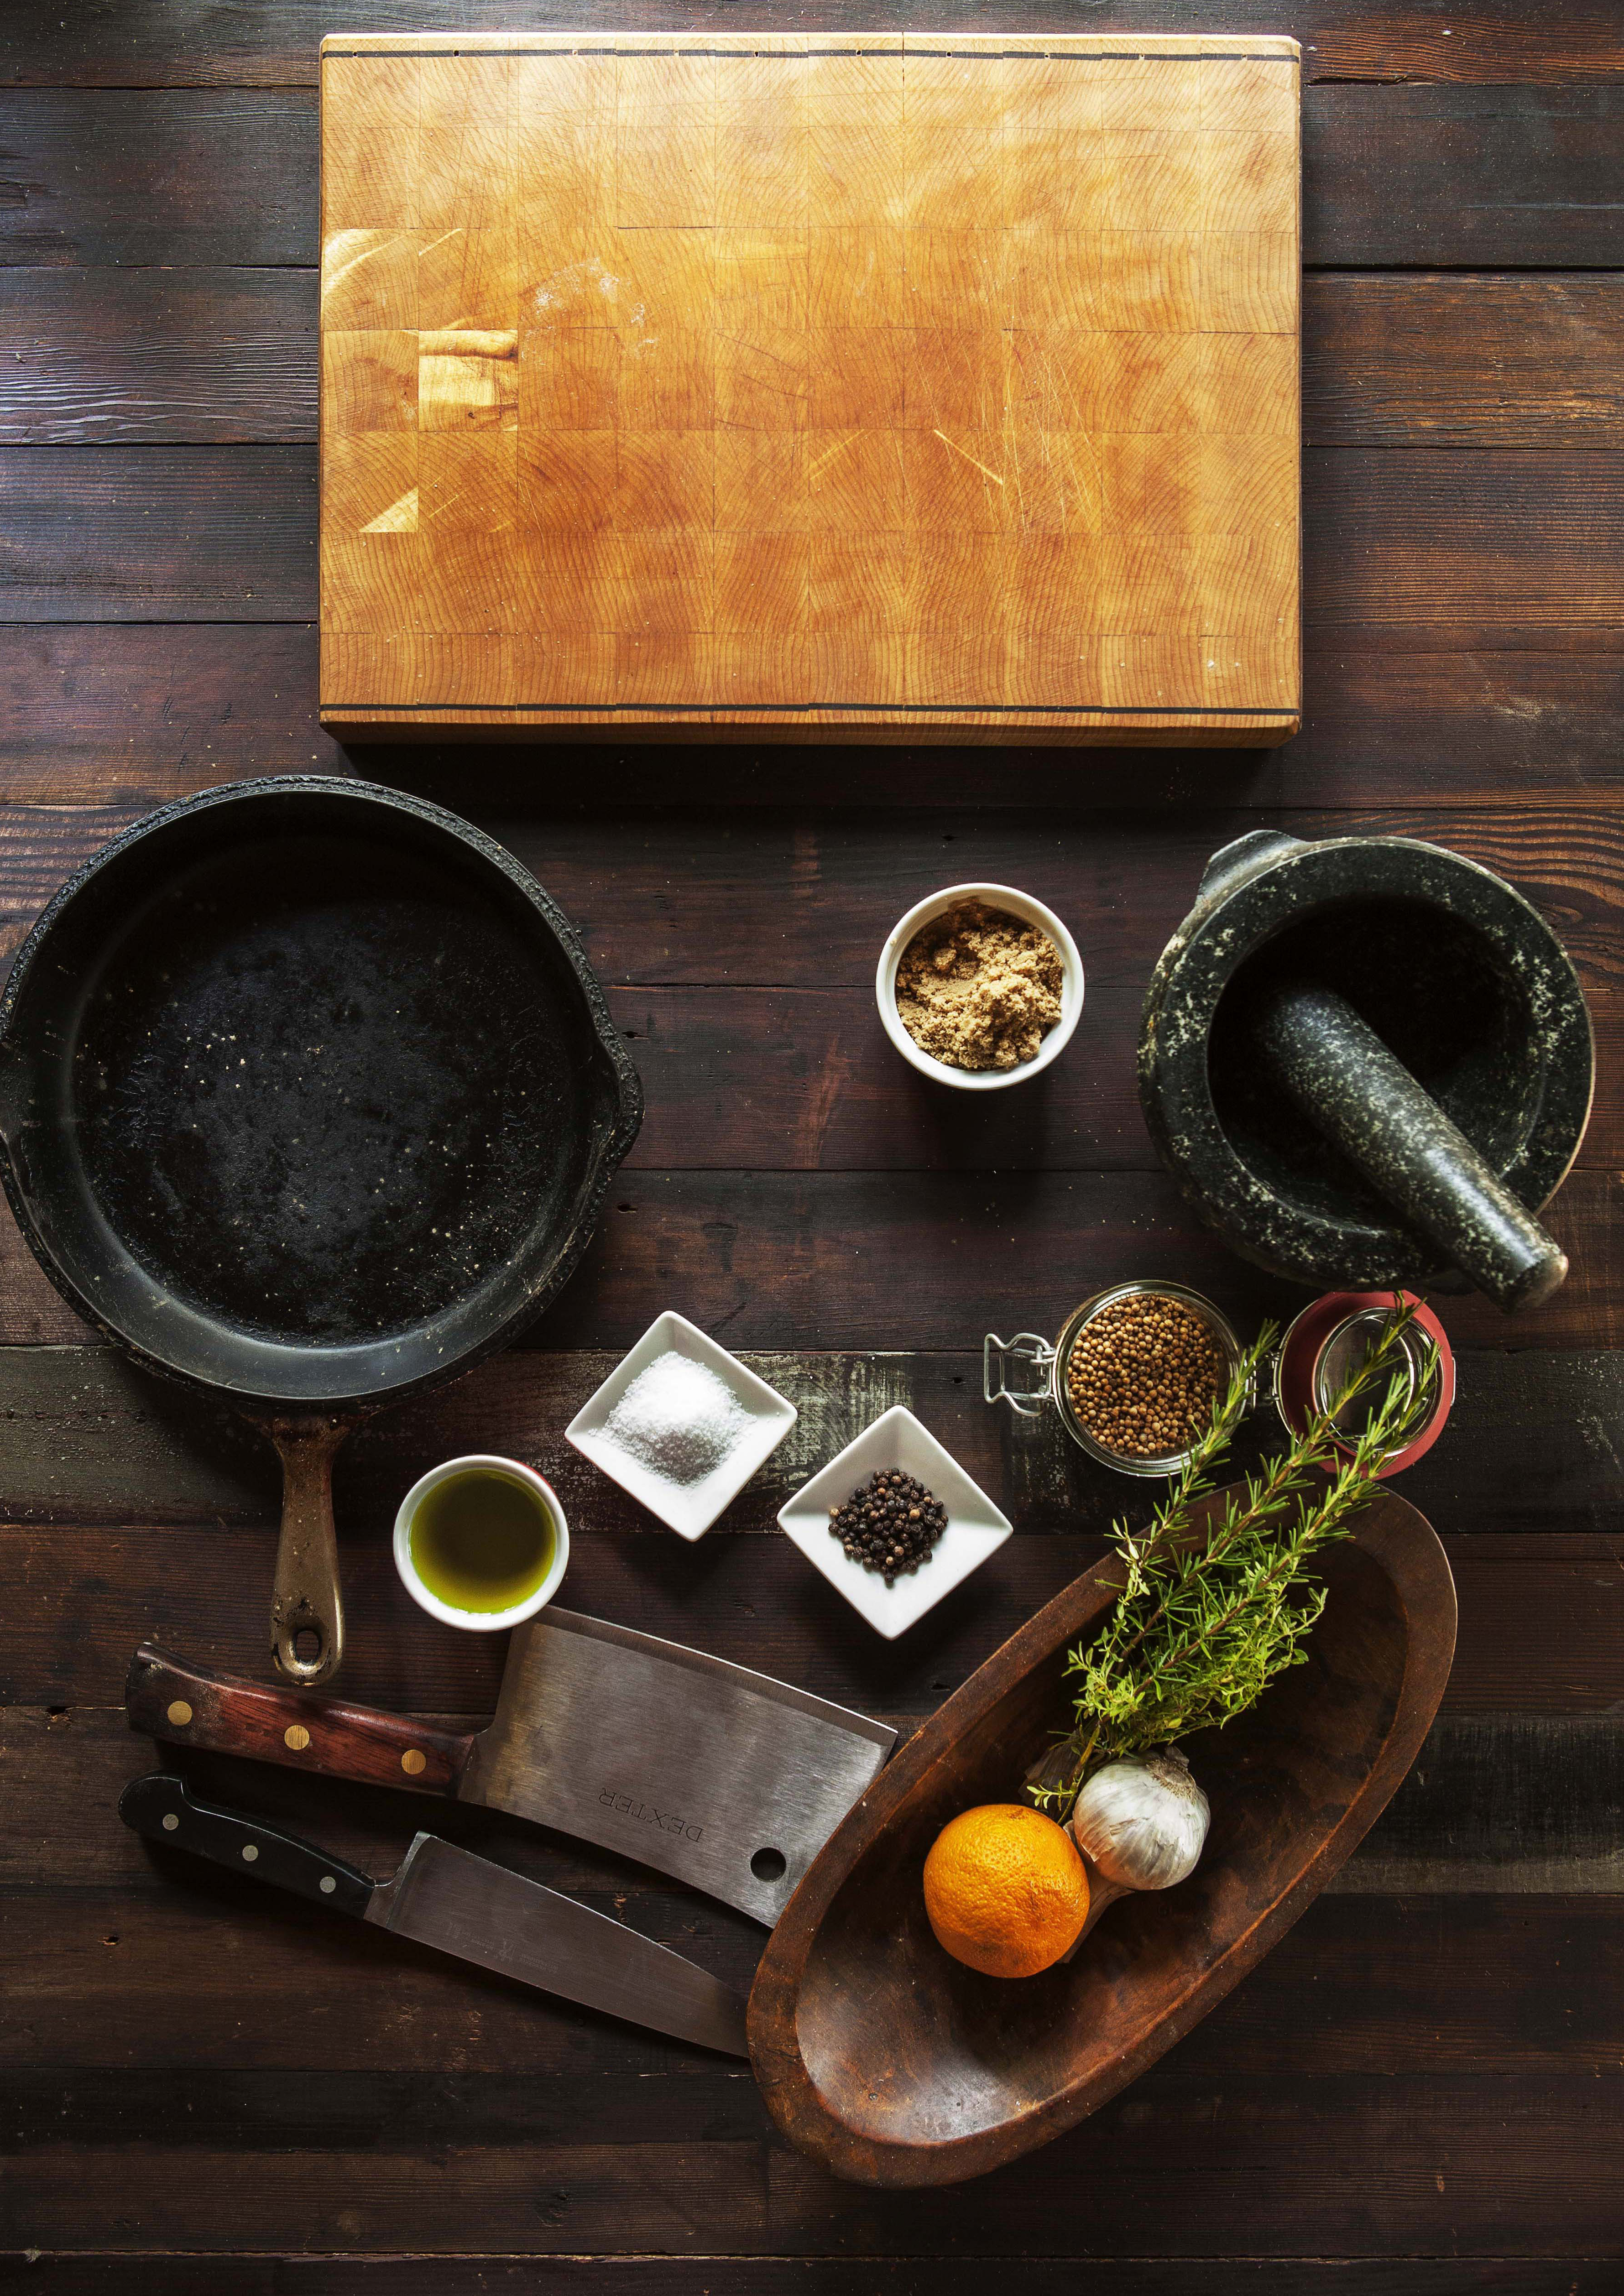
\includegraphics[width=\paperwidth, height=0.435\paperheight]{cover.jpg}
};
\end{tikzpicture}
\vspace*{0.356\paperheight}
\section*{\sectionformat Nome da Receita}
\addcontentsline{toc}{section}{Nome da Receita}
\vspace*{-0.1cm}
\begin{aemulticol}[width=0.495\textwidth,height=0.545\textheight]
	\begin{tabu} to 0.5\linewidth {X[l]X[r]}
	   \textit{Serve $3$ pessoas} & \textit{$430$ kcal}
	\end{tabu}\\
	\rule[0.5ex]{0.5\linewidth}{1pt}
	\vspace*{-0.7cm}
	\subsection*{\subsectionformat Teste}
	\vspace*{-0.15cm}
	\kant[1]
	\vspace*{-0.15cm}
	\subsection*{\subsectionformat Teste}
	\vspace*{-0.15cm}
	\kant[2-3]
	\vspace*{-0.15cm}
	\subsection*{\subsectionformat Teste}
	\vspace*{-0.15cm}
	\kant[3]
\end{aemulticol}

	\newpage
\noindent
\vspace*{-2.0cm}
\section*{\sectionformat Nome da Receita}
\addcontentsline{toc}{section}{Nome da Receita}
\vspace*{-0.1cm}
\begin{aemulticol}[width=0.495\textwidth,height=0.545\textheight]
	\begin{tabu} to 0.5\linewidth {X[l]X[r]}
	   \textit{Serve $3$ pessoas} & \textit{$430$ kcal}
	\end{tabu}\\
	\rule[0.5ex]{0.5\linewidth}{1pt}
	
	\vspace*{-0.3cm}
	\subsection*{\subsectionformat Ingredientes}
	\vspace*{-0.15cm}
	\begin{tabu} to 0.5\linewidth {X[l]X[l]}
	   $\bullet$ ingrediente com nome muito grande grande demais mesmo que cai pra outra linha & $\bullet$ ingrediente\\
	   $\bullet$ ingrediente & $\bullet$ ingrediente\\
	   $\bullet$ ingrediente & $\bullet$ ingrediente\\
	   $\bullet$ ingrediente & $\bullet$ ingrediente\\
	   $\bullet$ ingrediente & $\bullet$ ingrediente
	\end{tabu}

	\vspace*{-0.15cm}
	\subsection*{\subsectionformat Modo de Preparo}
	\vspace*{-0.15cm}
	$1.$  Passo 1\\
	$2.$  Passo 2\\
	$3.$  Passo 3\\
	$4.$  Passo 4\\
	$5.$  Passo 5\\
	$6.$  Passo 6\\
	$7.$  Passo 7\\
	$8.$  Passo 8\\
	$9.$  Passo 9\\
	$10.$ Passo 10\\
	$11.$ Passo 11\\
	$12.$ Passo 12\\
	$13.$ Passo 13\\
	$14.$ Passo 14\\
	$15.$ Passo 15\\
	$16.$ Passo 16\\
	$17.$ Passo 17\\
	$18.$ Passo 18\\
	$13.$ Passo 13\\
	$14.$ Passo 14\\
	$16.$ Passo 16\\
	$17.$ Passo 17\\
	$18.$ Passo 18\\
	$13.$ Passo 13\\
	$14.$ Passo 14\\
	$16.$ Passo 16\\
	$17.$ Passo 17\\
	$18.$ Passo 18\\
	$13.$ Passo 13\\
	$14.$ Passo 14\\
	$15.$ Passo 15\\
	$16.$ Passo 16\\
	$17.$ Passo 17\\
	$18.$ Passo 18\\
	$19.$ Passo 19	

	\vspace*{-0.15cm}
	\subsection*{\subsectionformat Dicas}
	\vspace*{-0.15cm}
	
	$\bullet$ Dica 1\\
	$\bullet$ Dica 2\\
	$\bullet$ Dica 3
	
	\vspace*{-0.15cm}
	\subsection*{\subsectionformat História}
	\vspace*{-0.15cm}
	\textit{Essa receita foi criada para testar o layout do livro e infelizmente, provavelmente nunca será feita. Coitada da receita.}
\end{aemulticol}
\begin{tikzpicture}[remember picture, overlay]
\node[anchor = south, inner sep = 0pt, outer sep = 0pt] at (current page.south) 
{
	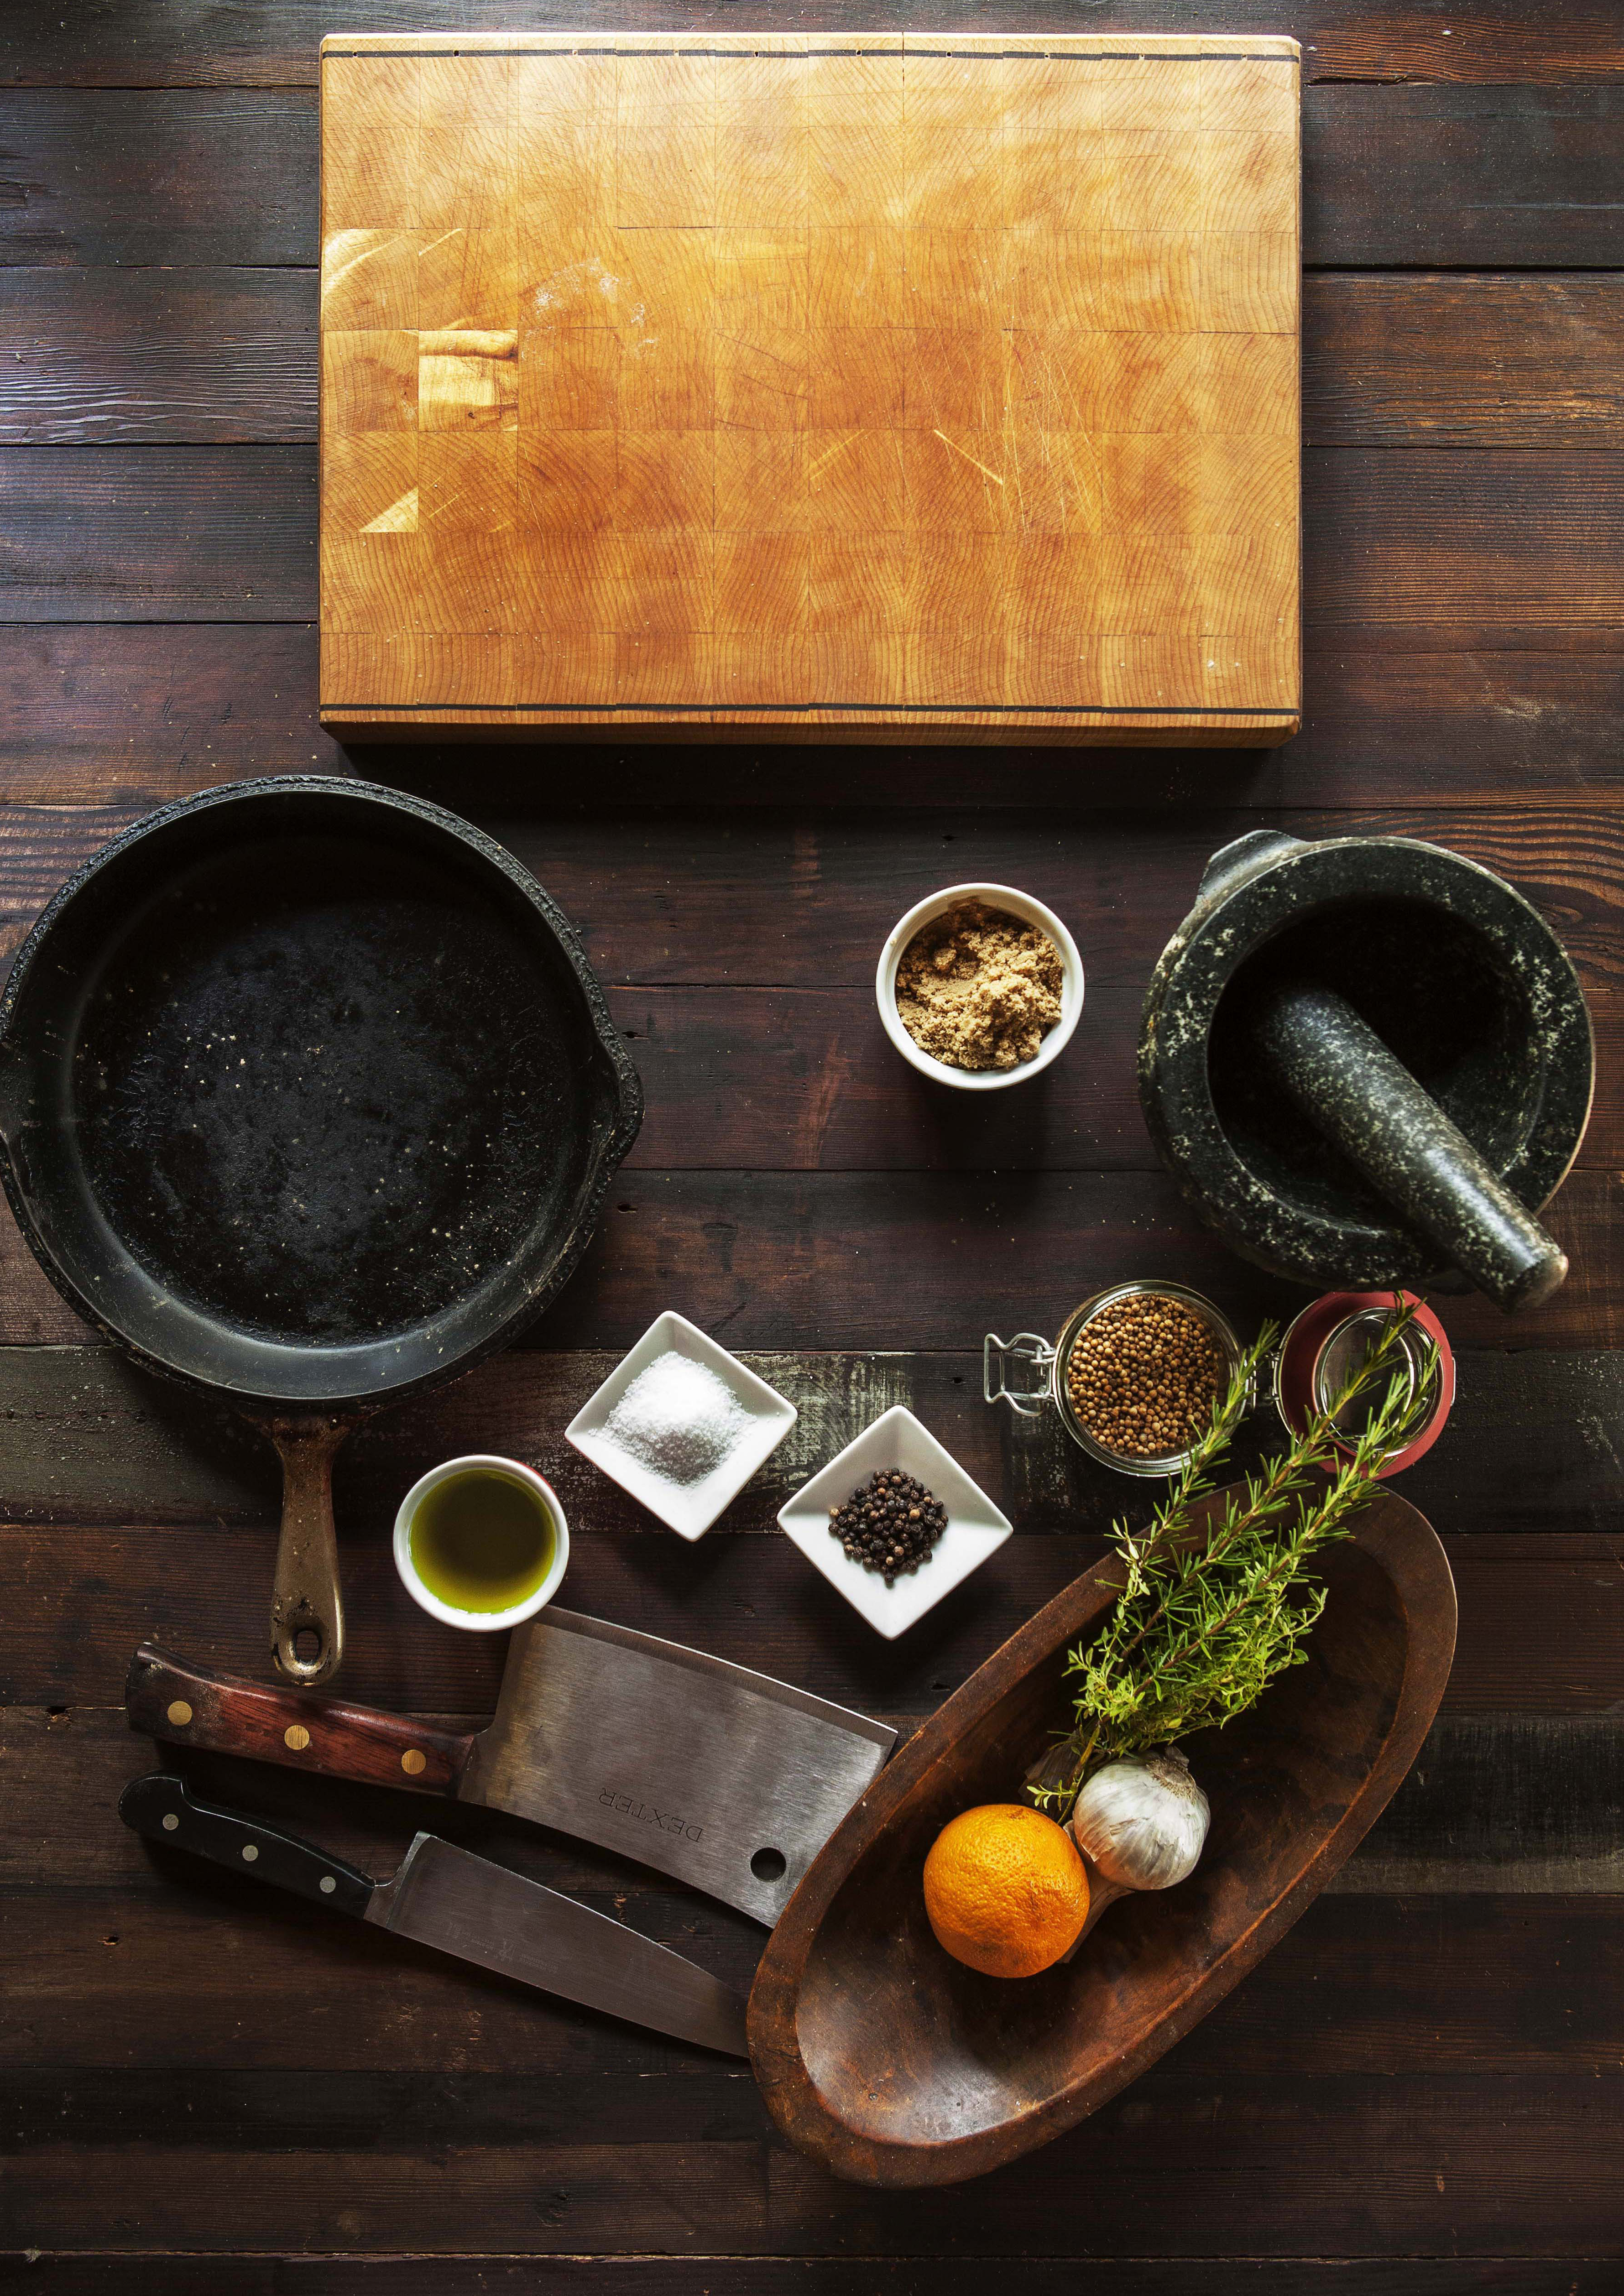
\includegraphics[width=\paperwidth, height=0.45\paperheight]{cover.jpg}
};
\end{tikzpicture}
	\newpage
\noindent
\begin{tikzpicture}[remember picture, overlay]
\node[anchor = north, inner sep = 0pt, outer sep = 0pt] at (current page.north) 
{
	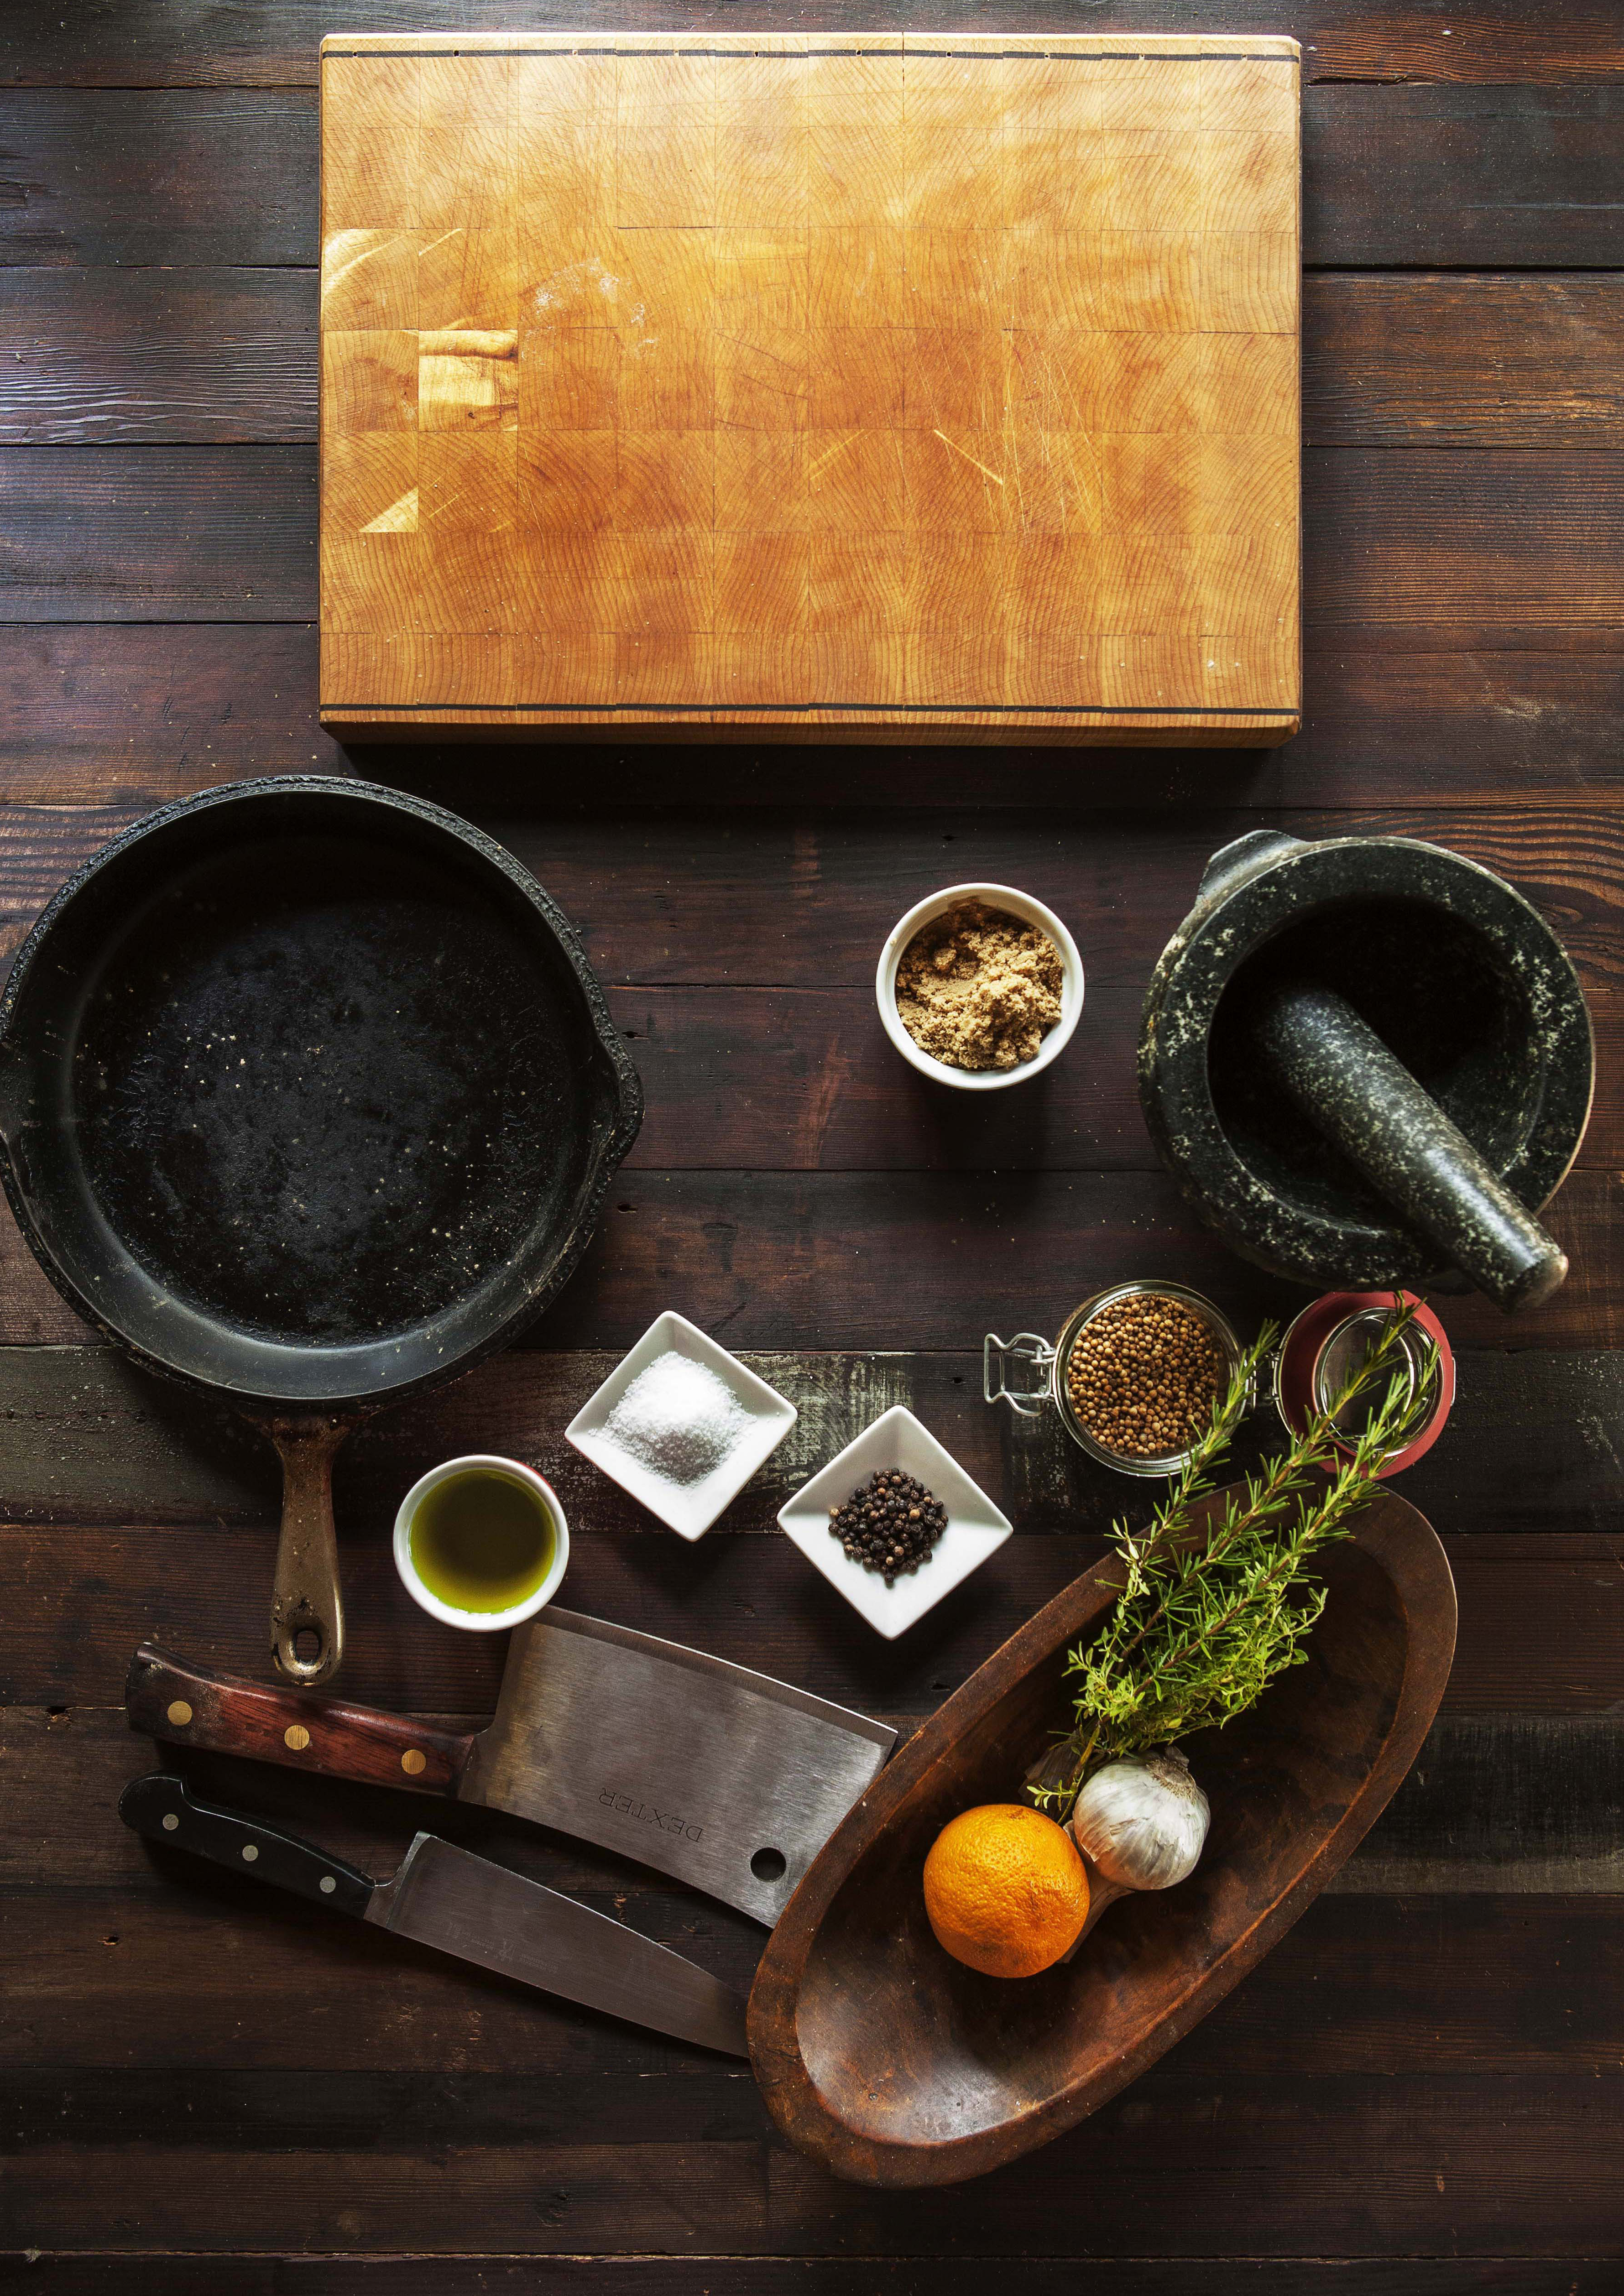
\includegraphics[width=\paperwidth, height=0.435\paperheight]{cover.jpg}
};
\end{tikzpicture}
\vspace*{0.356\paperheight}
\section*{\sectionformat Nome da Receita}
\addcontentsline{toc}{section}{Nome da Receita}
\vspace*{-0.1cm}
\begin{aemulticol}[width=0.495\textwidth,height=0.545\textheight]
	\begin{tabu} to 0.5\linewidth {X[l]X[r]}
	   \textit{Serve $3$ pessoas} & \textit{$430$ kcal}
	\end{tabu}\\
	\rule[0.5ex]{0.5\linewidth}{1pt}
	\vspace*{-0.7cm}
	\subsection*{\subsectionformat Teste}
	\vspace*{-0.15cm}
	\kant[1]
	\vspace*{-0.15cm}
	\subsection*{\subsectionformat Teste}
	\vspace*{-0.15cm}
	\kant[2-3]
	\vspace*{-0.15cm}
	\subsection*{\subsectionformat Teste}
	\vspace*{-0.15cm}
	\kant[3]
\end{aemulticol}

	\newpage
\noindent
\vspace*{-2.0cm}
\section*{\sectionformat Nome da Receita}
\addcontentsline{toc}{section}{Nome da Receita}
\vspace*{-0.1cm}
\begin{aemulticol}[width=0.495\textwidth,height=0.545\textheight]
	\begin{tabu} to 0.5\linewidth {X[l]X[r]}
	   \textit{Serve $3$ pessoas} & \textit{$430$ kcal}
	\end{tabu}\\
	\rule[0.5ex]{0.5\linewidth}{1pt}
	
	\vspace*{-0.3cm}
	\subsection*{\subsectionformat Ingredientes}
	\vspace*{-0.15cm}
	\begin{tabu} to 0.5\linewidth {X[l]X[l]}
	   $\bullet$ ingrediente com nome muito grande grande demais mesmo que cai pra outra linha & $\bullet$ ingrediente\\
	   $\bullet$ ingrediente & $\bullet$ ingrediente\\
	   $\bullet$ ingrediente & $\bullet$ ingrediente\\
	   $\bullet$ ingrediente & $\bullet$ ingrediente\\
	   $\bullet$ ingrediente & $\bullet$ ingrediente
	\end{tabu}

	\vspace*{-0.15cm}
	\subsection*{\subsectionformat Modo de Preparo}
	\vspace*{-0.15cm}
	$1.$  Passo 1\\
	$2.$  Passo 2\\
	$3.$  Passo 3\\
	$4.$  Passo 4\\
	$5.$  Passo 5\\
	$6.$  Passo 6\\
	$7.$  Passo 7\\
	$8.$  Passo 8\\
	$9.$  Passo 9\\
	$10.$ Passo 10\\
	$11.$ Passo 11\\
	$12.$ Passo 12\\
	$13.$ Passo 13\\
	$14.$ Passo 14\\
	$15.$ Passo 15\\
	$16.$ Passo 16\\
	$17.$ Passo 17\\
	$18.$ Passo 18\\
	$13.$ Passo 13\\
	$14.$ Passo 14\\
	$16.$ Passo 16\\
	$17.$ Passo 17\\
	$18.$ Passo 18\\
	$13.$ Passo 13\\
	$14.$ Passo 14\\
	$16.$ Passo 16\\
	$17.$ Passo 17\\
	$18.$ Passo 18\\
	$13.$ Passo 13\\
	$14.$ Passo 14\\
	$15.$ Passo 15\\
	$16.$ Passo 16\\
	$17.$ Passo 17\\
	$18.$ Passo 18\\
	$19.$ Passo 19	

	\vspace*{-0.15cm}
	\subsection*{\subsectionformat Dicas}
	\vspace*{-0.15cm}
	
	$\bullet$ Dica 1\\
	$\bullet$ Dica 2\\
	$\bullet$ Dica 3
	
	\vspace*{-0.15cm}
	\subsection*{\subsectionformat História}
	\vspace*{-0.15cm}
	\textit{Essa receita foi criada para testar o layout do livro e infelizmente, provavelmente nunca será feita. Coitada da receita.}
\end{aemulticol}
\begin{tikzpicture}[remember picture, overlay]
\node[anchor = south, inner sep = 0pt, outer sep = 0pt] at (current page.south) 
{
	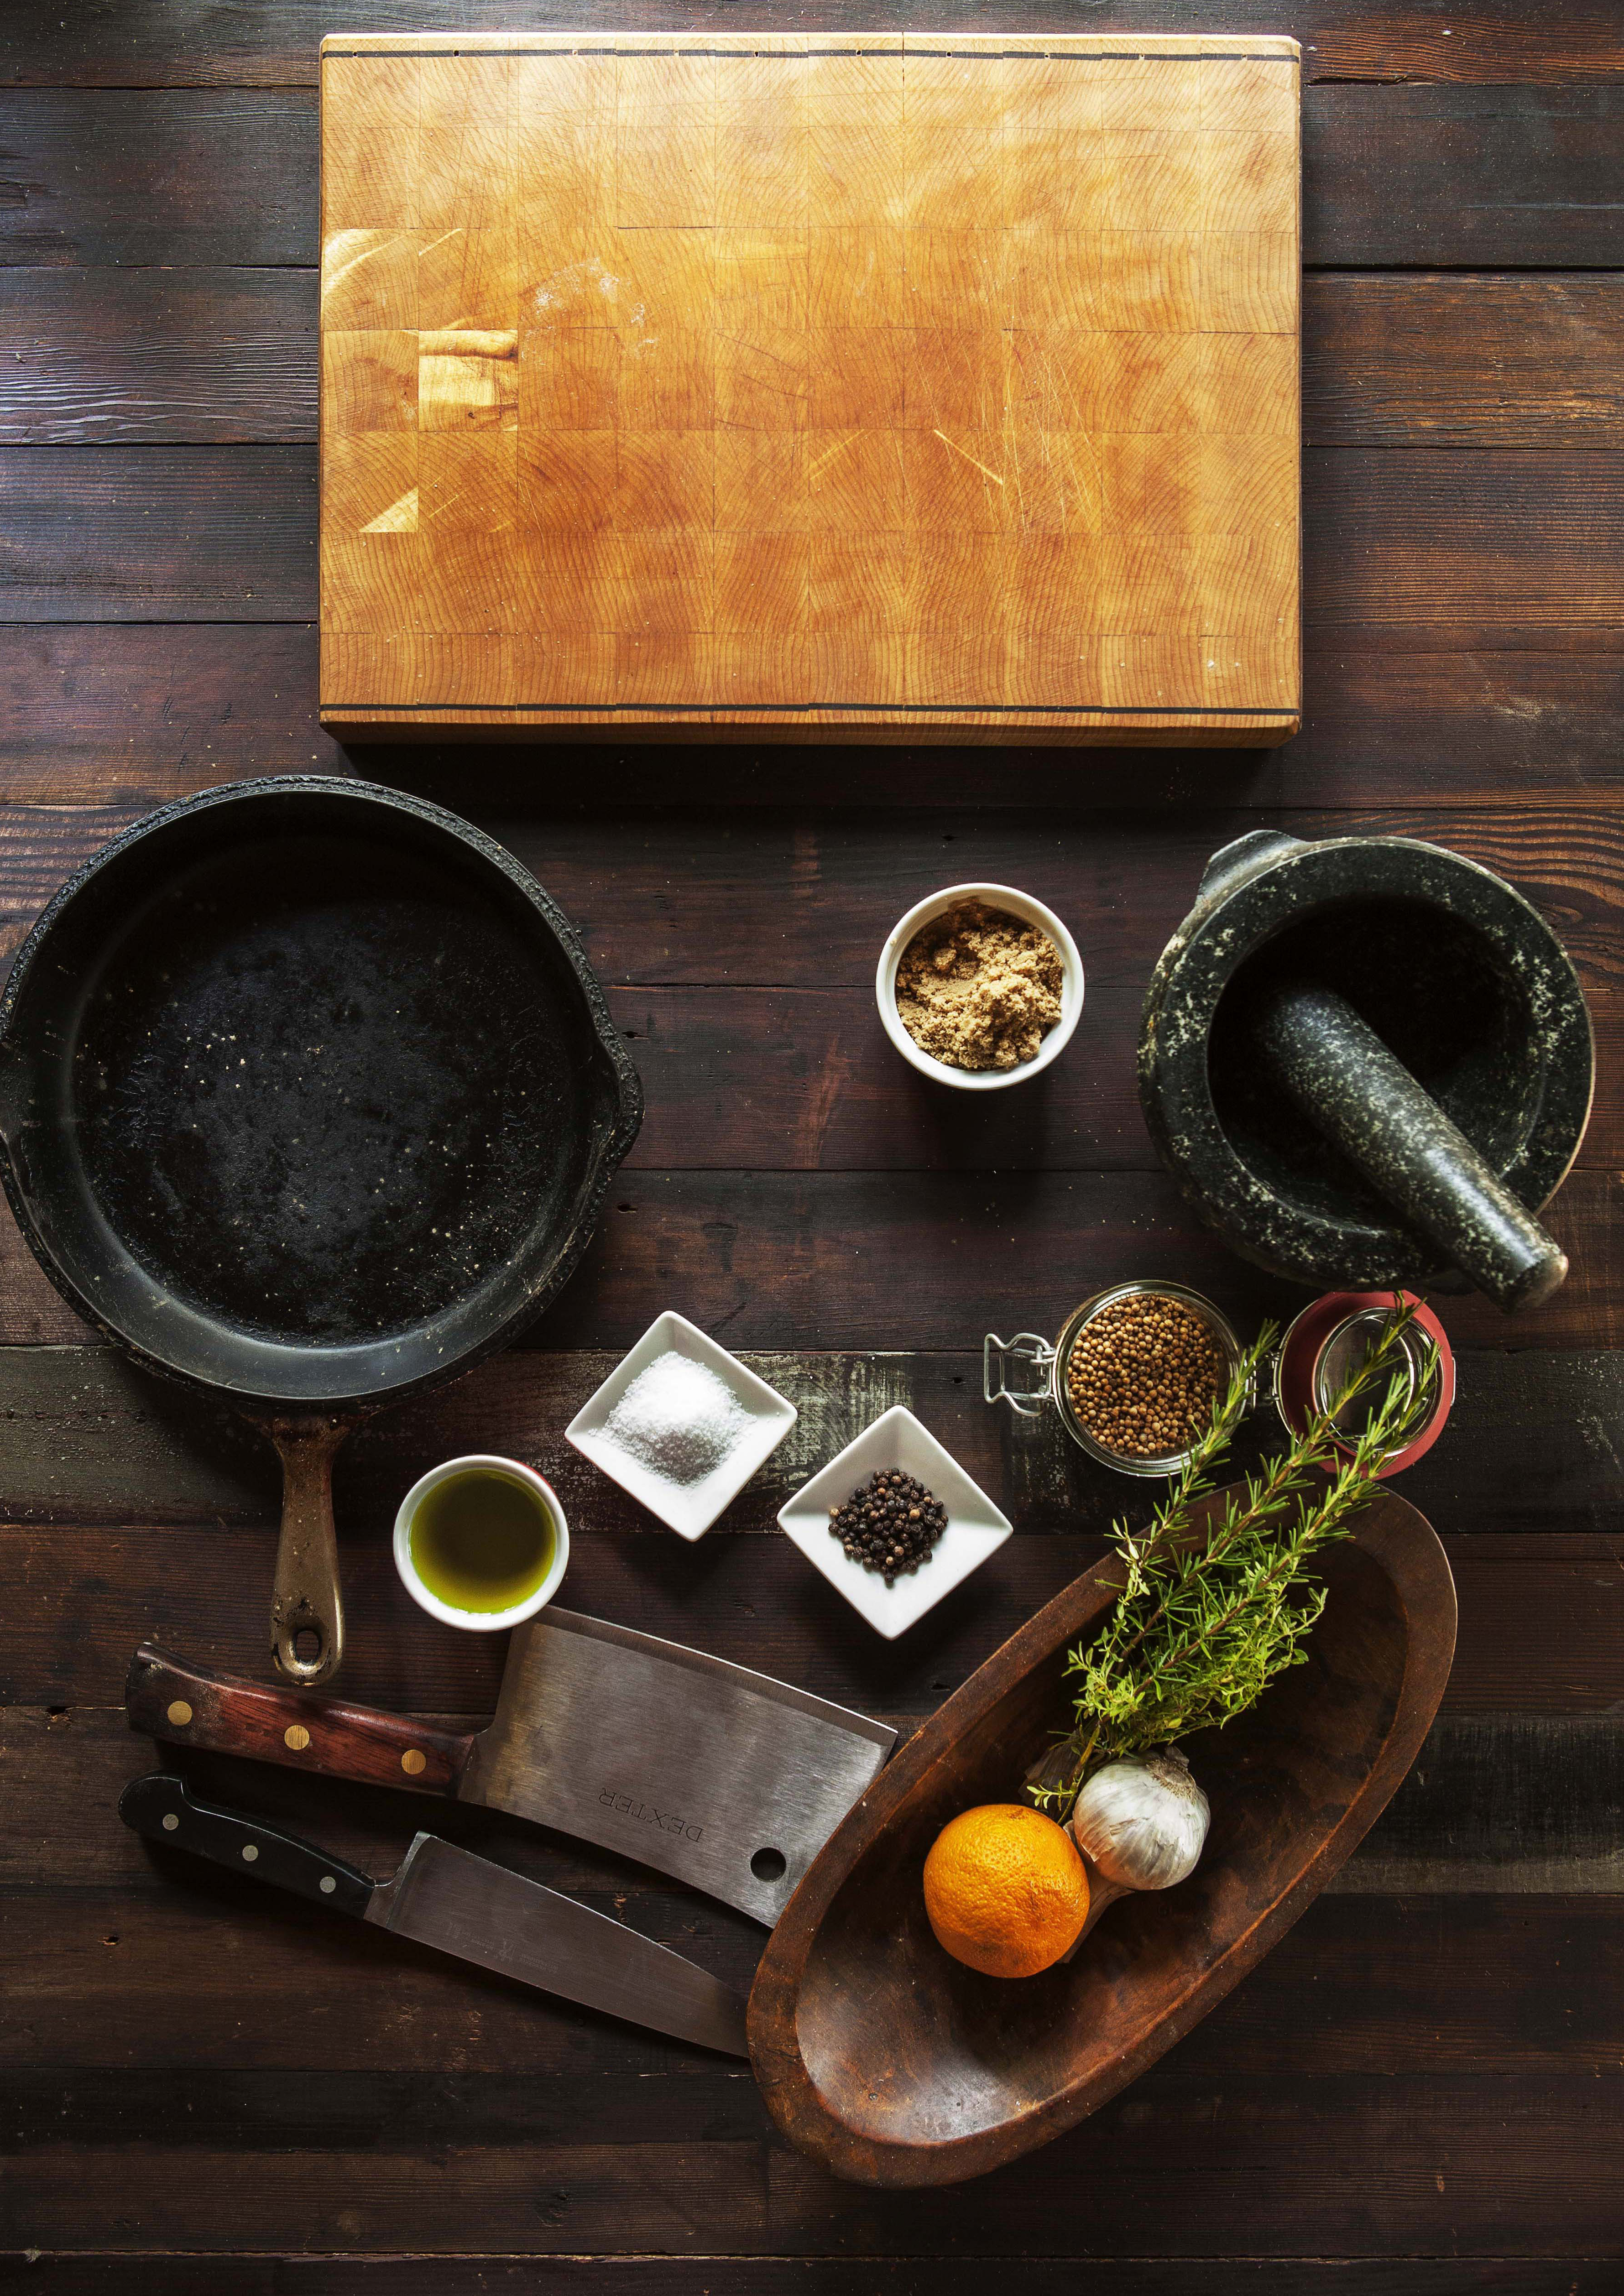
\includegraphics[width=\paperwidth, height=0.45\paperheight]{cover.jpg}
};
\end{tikzpicture}
	\newpage
\noindent
\begin{tikzpicture}[remember picture, overlay]
\node[anchor = north, inner sep = 0pt, outer sep = 0pt] at (current page.north) 
{
	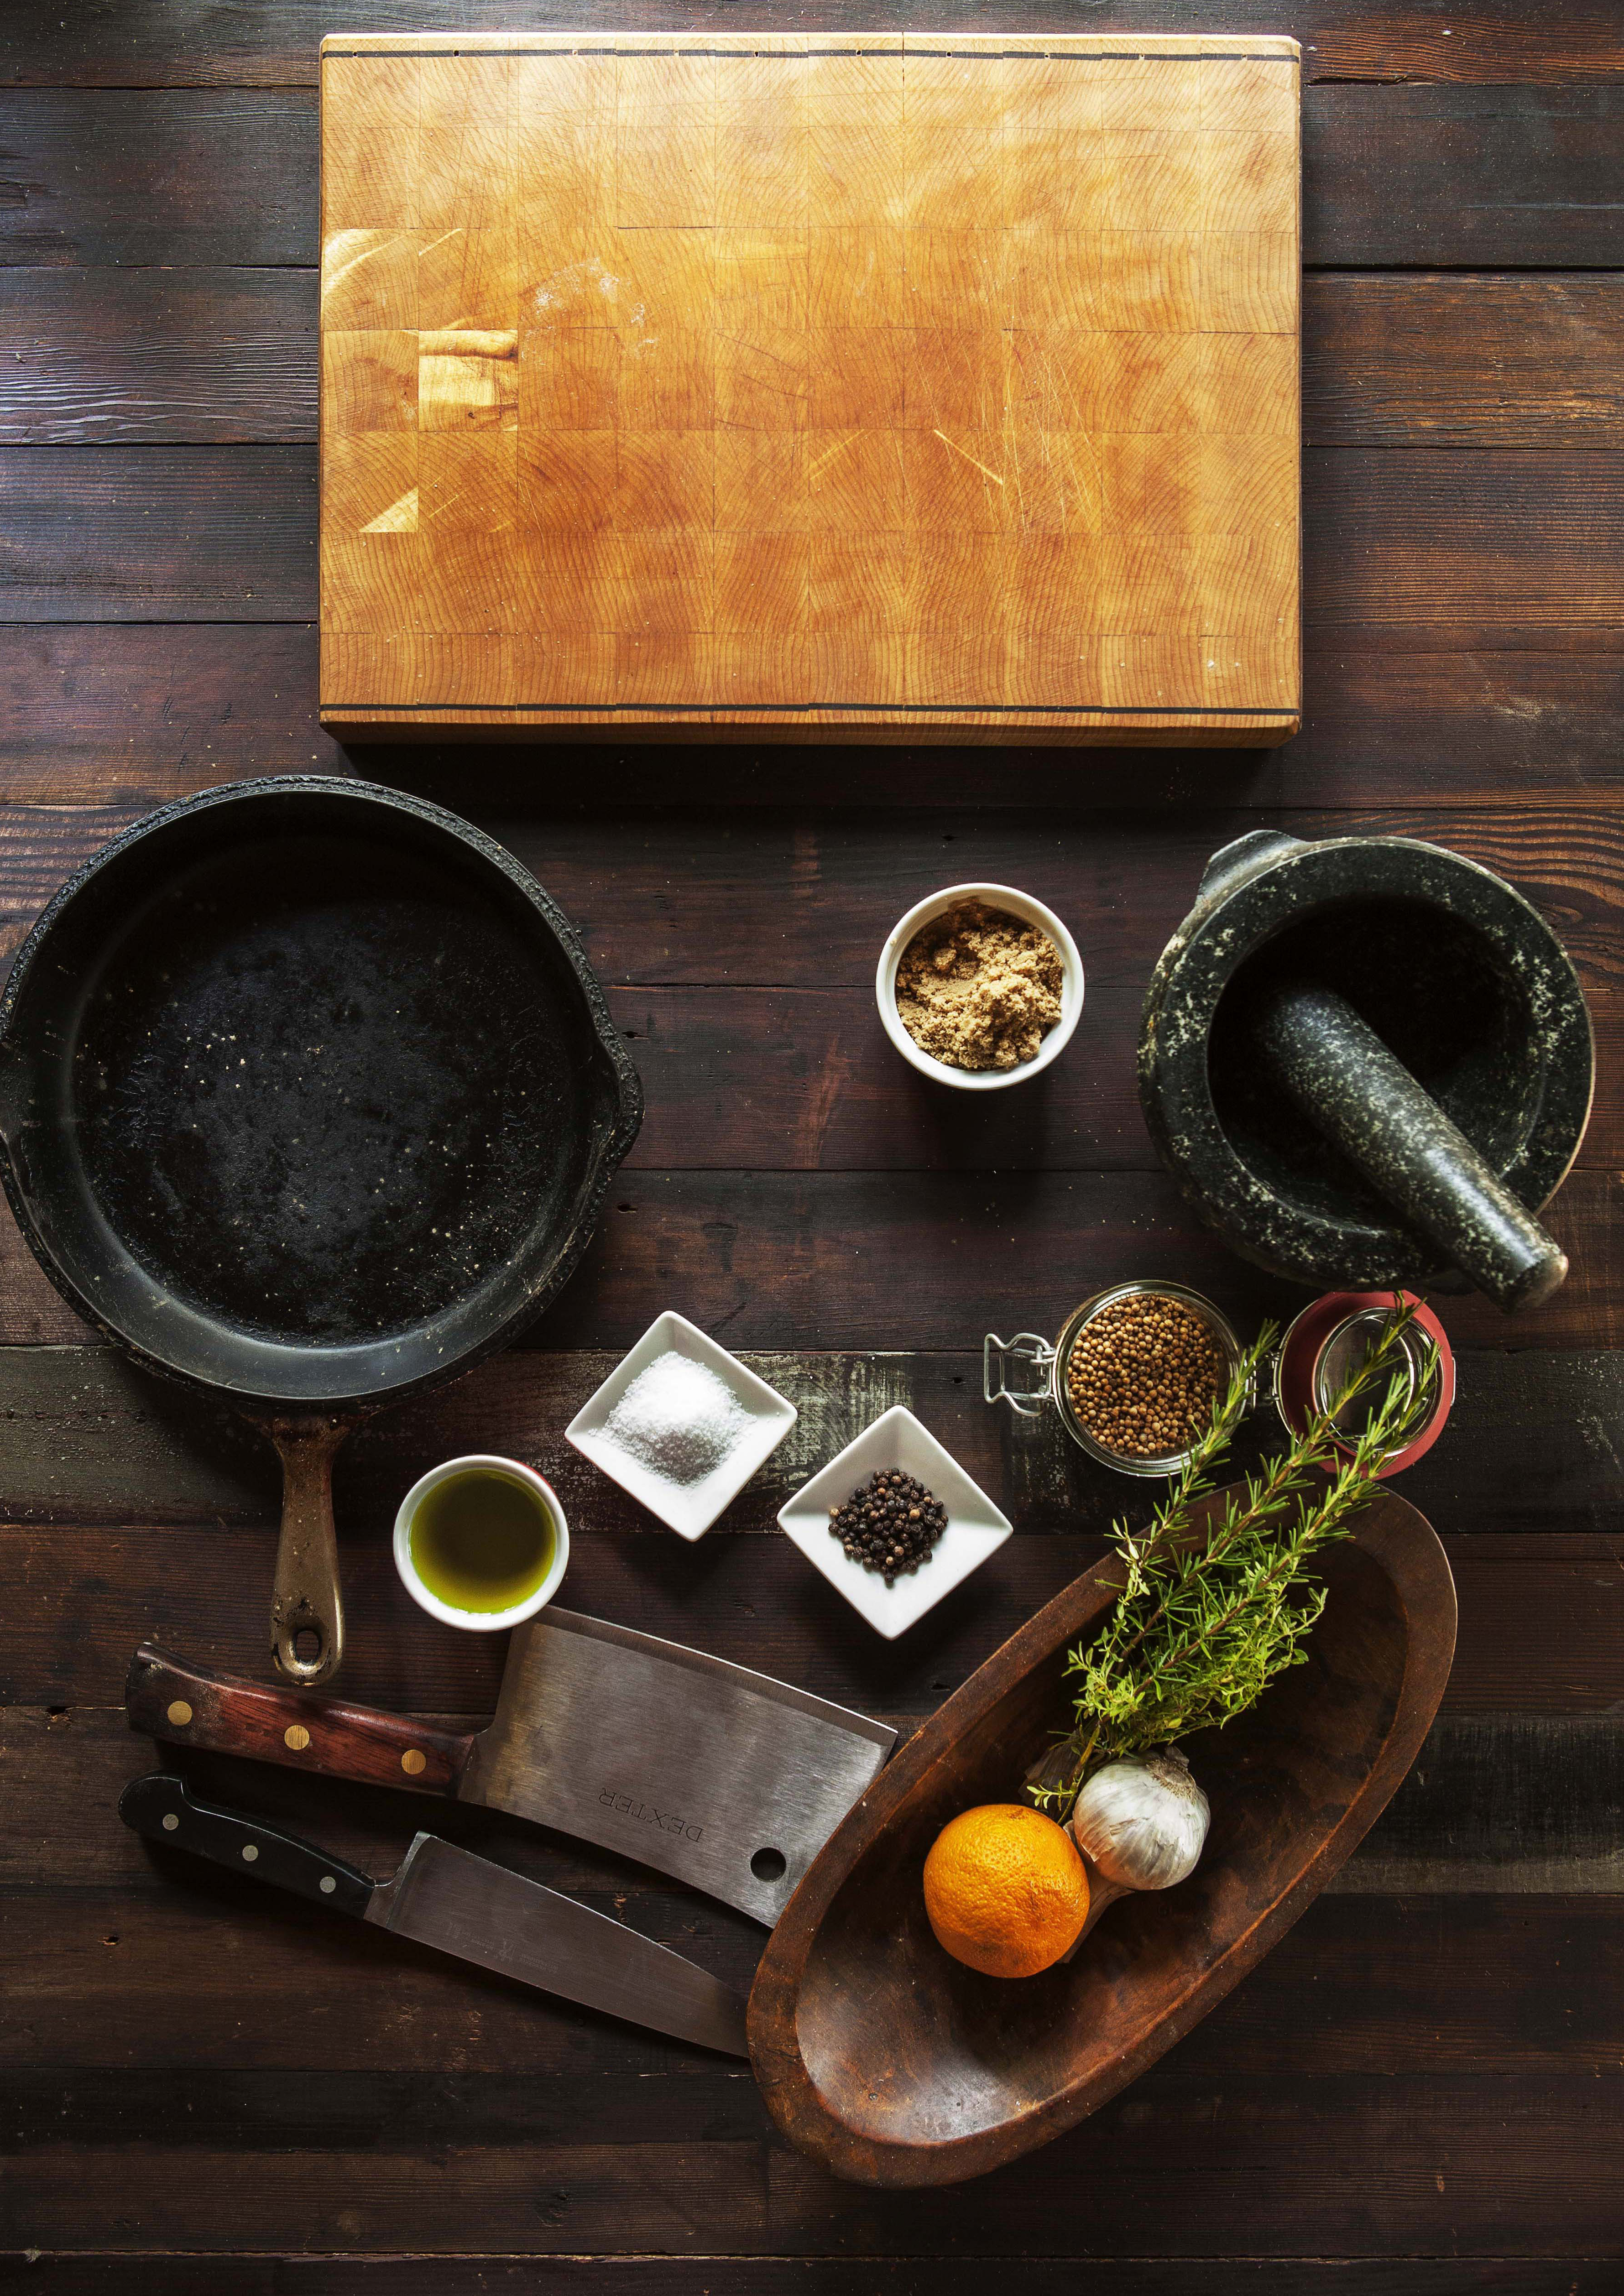
\includegraphics[width=\paperwidth, height=0.435\paperheight]{cover.jpg}
};
\end{tikzpicture}
\vspace*{0.356\paperheight}
\section*{\sectionformat Nome da Receita}
\addcontentsline{toc}{section}{Nome da Receita}
\vspace*{-0.1cm}
\begin{aemulticol}[width=0.495\textwidth,height=0.545\textheight]
	\begin{tabu} to 0.5\linewidth {X[l]X[r]}
	   \textit{Serve $3$ pessoas} & \textit{$430$ kcal}
	\end{tabu}\\
	\rule[0.5ex]{0.5\linewidth}{1pt}
	\vspace*{-0.7cm}
	\subsection*{\subsectionformat Teste}
	\vspace*{-0.15cm}
	\kant[1]
	\vspace*{-0.15cm}
	\subsection*{\subsectionformat Teste}
	\vspace*{-0.15cm}
	\kant[2-3]
	\vspace*{-0.15cm}
	\subsection*{\subsectionformat Teste}
	\vspace*{-0.15cm}
	\kant[3]
\end{aemulticol}


\end{document}